\section{Translator}\label{sec:translator}

We developed a Java-based tool to translate \conesc structures to plain nesC and
compile them into a binary. The translator performs two passes through the
project, it reads a \emph{Makefile} to get the main configuration component of
the project and briefly scans the components tree. During the second pass the
tool performs a parsing by using of Javacc libraries, and analyzes each
component and -- having the information about all declared \emph{contexts} and
\emph{context groups} -- generates nesC source code. At the end of generation,
our tool invokes nesC compiler and displays its output. When compilation is
finished, the tool removes generated files from the file-system.

\putfigure{caption=\conesc translator diagram.,label=fig:ctd}{
 \centering
 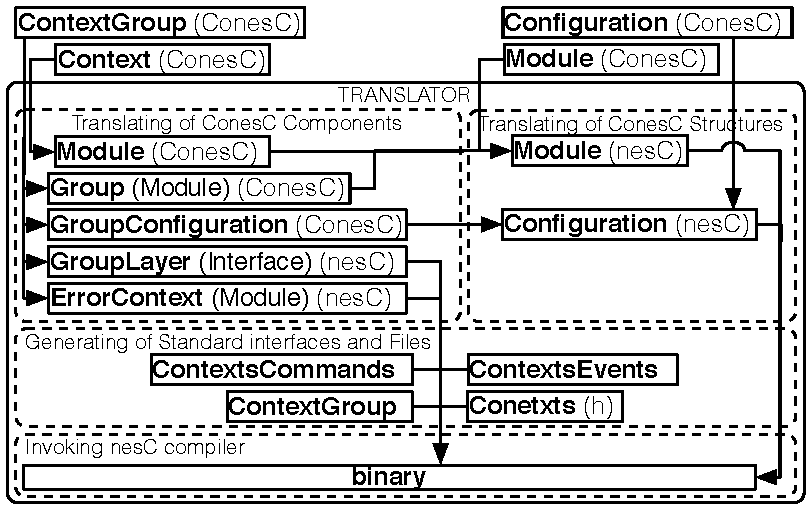
\includegraphics[width=\columnwidth]{pdf/translator}
}

\putfigure{caption=Hierarchy of generated components.,label=fig:gfh}{
 \centering
 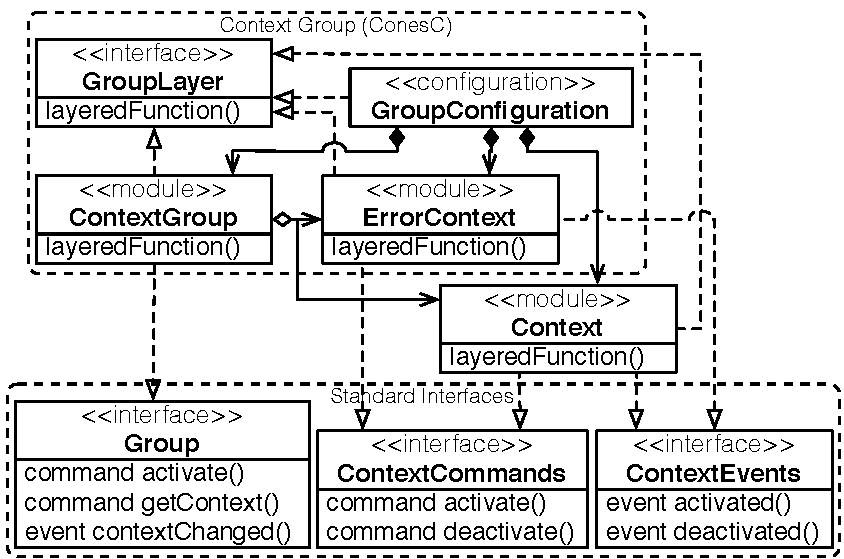
\includegraphics[width=\columnwidth]{pdf/architecture}
}

The input of the translator contains of four types of components: context
group, context, module and configuration, as shown in
Fig.~\ref{fig:ctd}. The latter two possibly contain \conesc structures and do
not define the architecture of the project, while the former two are surely
written in \conesc and base a skeleton of software. 

The hierarchy of generated based on \emph{context group} components is displayed
in Fig.~\ref{fig:gfh}. \emph{GroupLayer} -- a basic interface for all generated
components -- declares a \emph{layered function}. \emph{GroupConfiguration} is a
main component, which instantiates \emph{ConetxtGroup} and declared
\emph{contexts}, and glue them together. The former implements all the internal
logic to operate by \emph{contexts} and enable behavioral variation.
\emph{ErrorContext} module is generated if it was not declared in the
\emph{context group}. \emph{Context} is translated into module by adding
standard functions and implementation of \emph{group layer} interface mentioned
above.

The generated components and written by a developer modules are translated then
from \conesc into nesC. After that the translator generates standard interfaces
for additional functionality -- e.g. activation and deactivation of contexts --
for \emph{ContextGroup} and \emph{contexts}. \emph{Contexts.h} is a definition
of all the contexts in the projects. The last step is invoking the nesC compiler
to build a binary by using all the generated and transformed components.
